% vLLM V1: one mixed (chunked-prefill + decode + prefill) batch -> FlashAttention inputs.
% Grounded in vllm @ 4c2d277643e217344056e1d2c42115d5f005912f:
%   GR = vllm/v1/worker/gpu_model_runner.py
%   BT = vllm/v1/worker/block_table.py
%   FA = vllm/v1/attention/backends/flash_attn.py
\documentclass[border=10pt]{standalone}
\usepackage{amsmath,amssymb}
\usepackage[table]{xcolor}
\usepackage{tikz}
\usetikzlibrary{arrows.meta,backgrounds,calc,fit,positioning,decorations.pathreplacing}

\definecolor{ink}{HTML}{252525}
\definecolor{rulegray}{HTML}{9A9A9A}
\definecolor{rcA}{HTML}{F2BDBD} % R0  chunked prefill (pink)
\definecolor{rcB}{HTML}{BFE0BF} % R1  decode (green)
\definecolor{rcC}{HTML}{BCD5EE} % R2  new prefill (blue)
\definecolor{oldkv}{HTML}{EDEDED}
\definecolor{padc}{HTML}{D6D6D6}
\definecolor{paperyellow}{HTML}{F5F2C8}
\definecolor{paperpeach}{HTML}{FBEBD6}
\definecolor{paperlavender}{HTML}{E9E4F1}

% ---- parameters -----------------------------------------------------------
\def\tx{8.9}    % x of first flattened-token cell
\def\tw{1.70}   % flattened-token cell width
\def\cx{0.6}    % x of KV block 0
\def\cw{0.62}   % KV slot width
\def\bg{0.22}   % gap between KV blocks
\def\gw{0.62}   % attention-grid cell size

\newcommand{\src}[1]{{\ttfamily\scriptsize\color{ink!65}#1}}
\newcommand{\code}[1]{{\ttfamily #1}}

\begin{document}
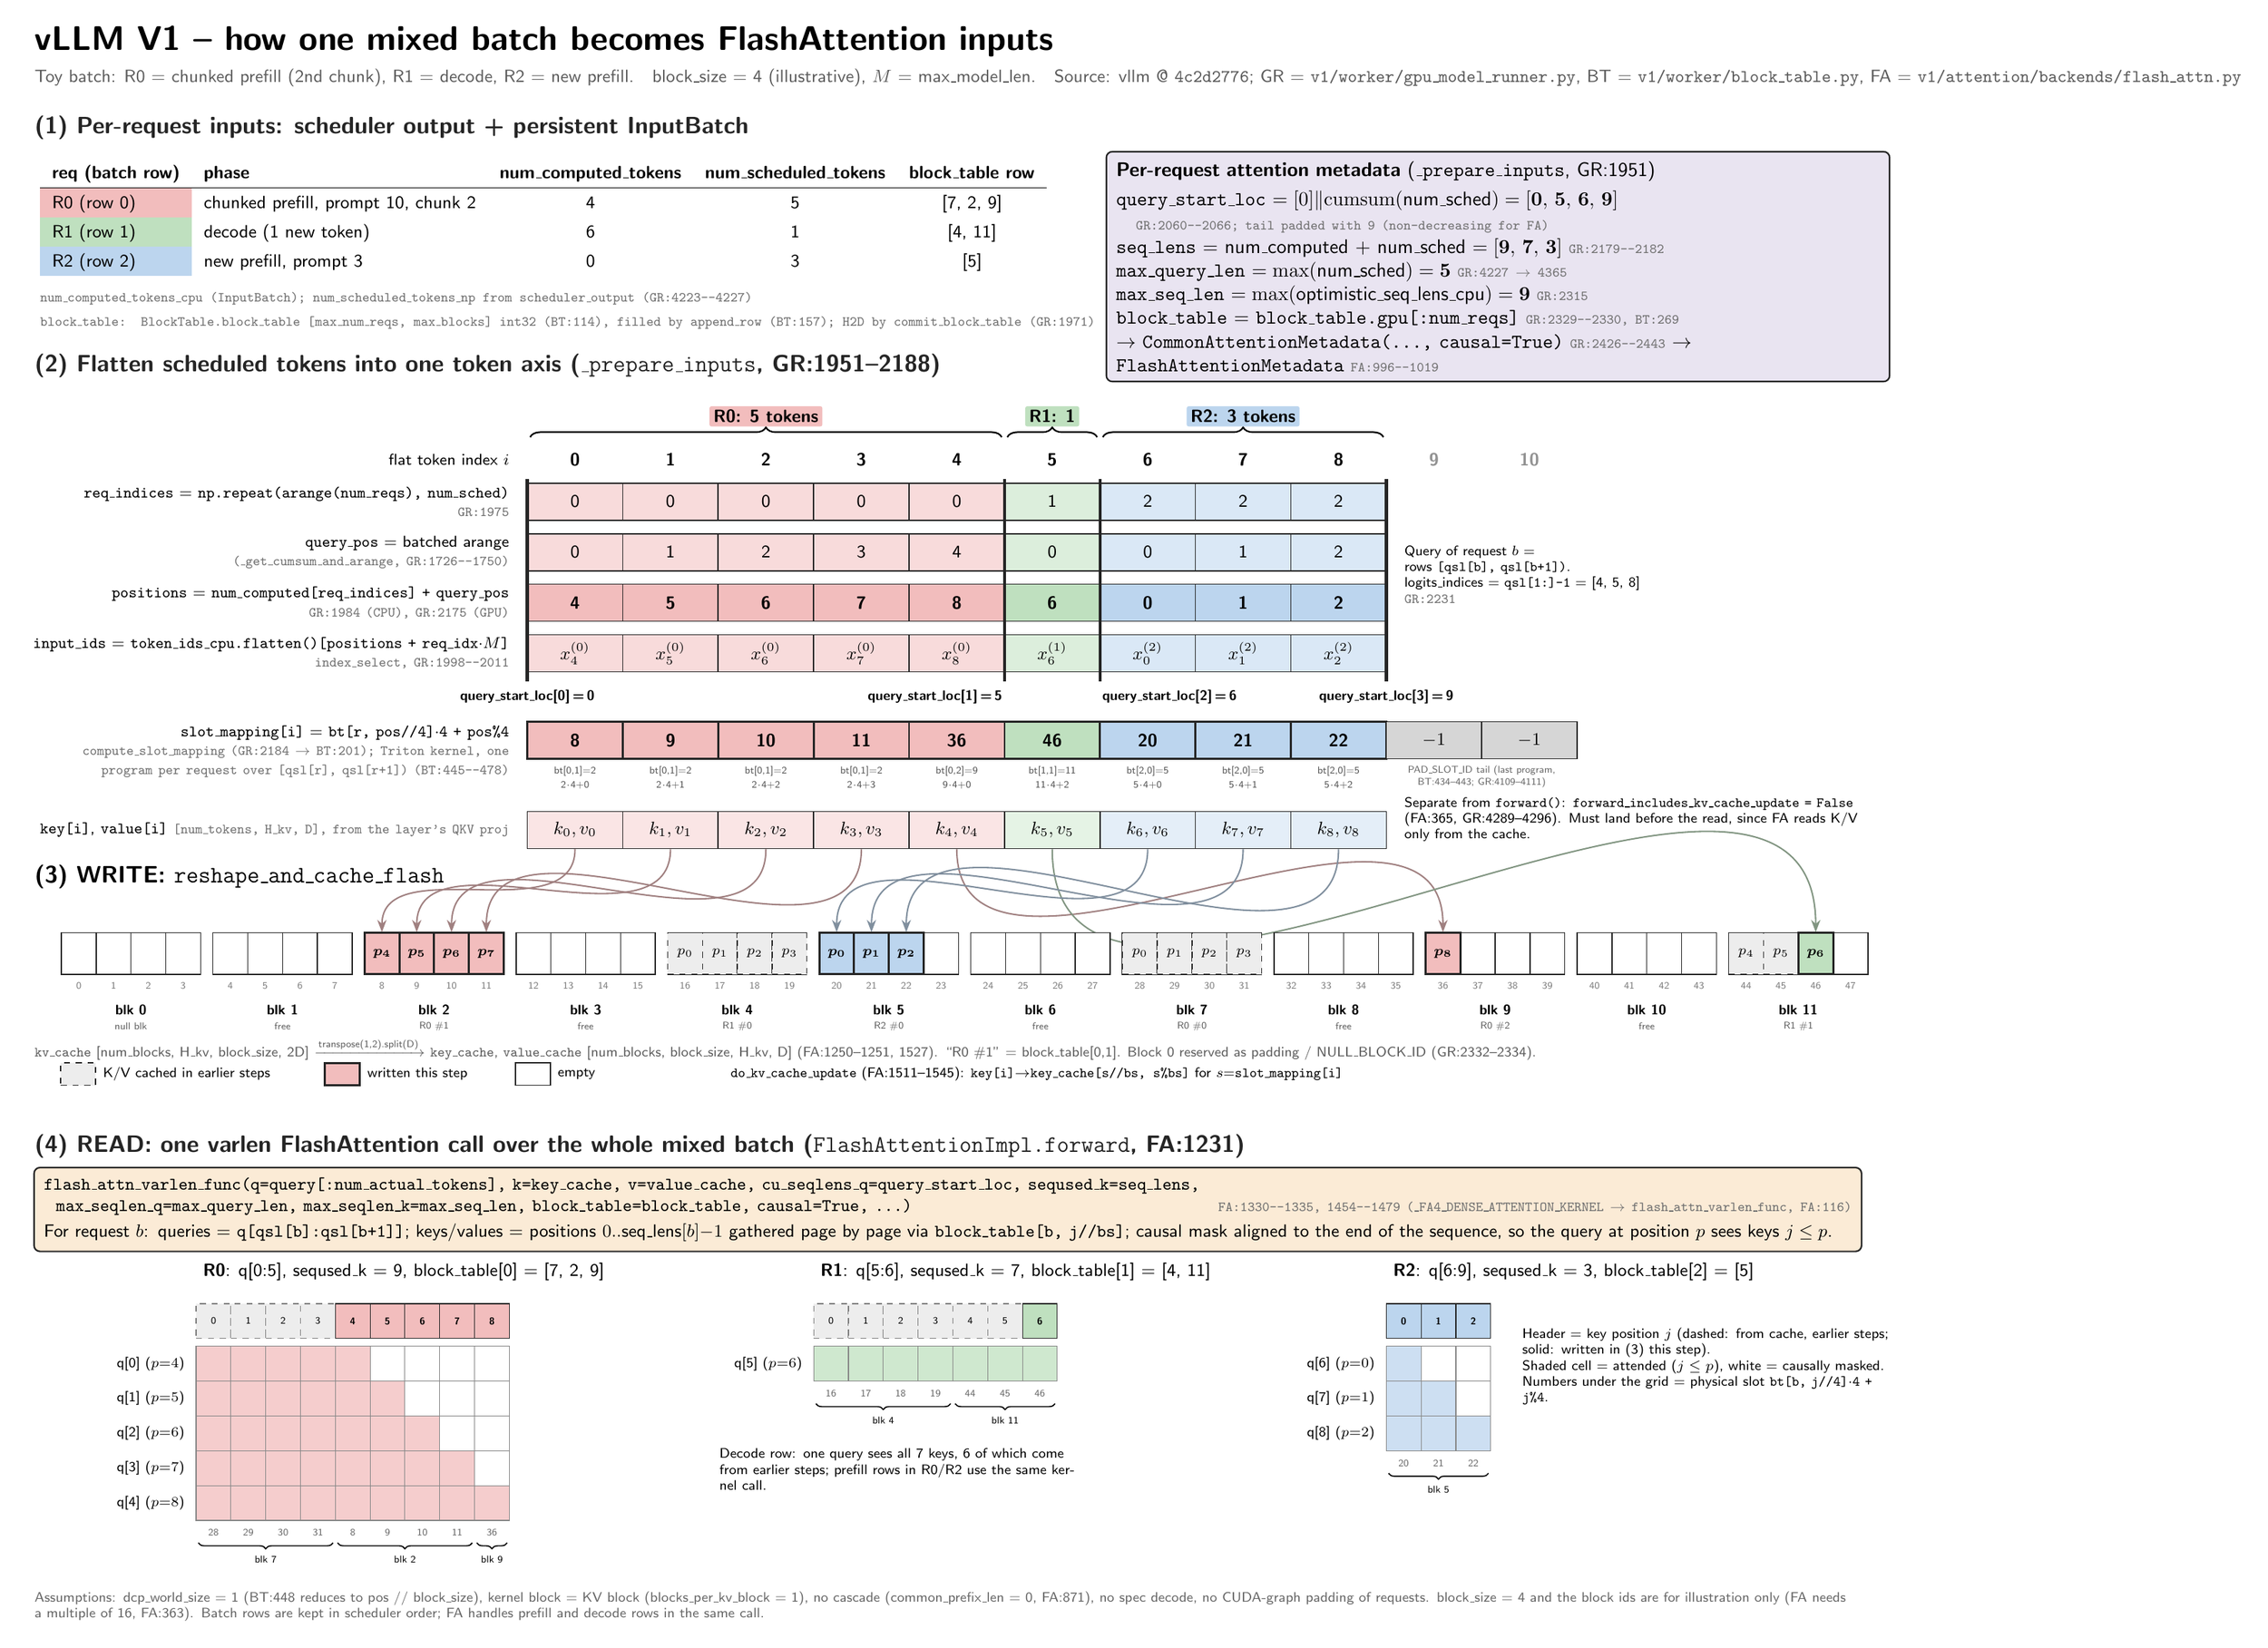
\begin{tikzpicture}[
  font=\sffamily,
  >={Stealth[length=2.2mm]},
  tok/.style={draw=ink,line width=.6pt,minimum width=\tw cm,minimum height=.66cm,inner sep=0pt,font=\sffamily\small},
  slot/.style={draw=ink,line width=.55pt,minimum width=\cw cm,minimum height=.74cm,inner sep=0pt,font=\sffamily\scriptsize},
  gcell/.style={draw=ink!55,line width=.4pt,minimum width=\gw cm,minimum height=\gw cm,inner sep=0pt,font=\sffamily\tiny},
  rowlab/.style={anchor=east,align=right,text width=8.6cm,font=\sffamily\footnotesize},
  sec/.style={anchor=north west,font=\sffamily\bfseries\large,text=ink},
  box/.style={draw=ink,rounded corners=3pt,line width=.8pt,align=left,inner sep=5pt},
  wr/.style={->,line width=.75pt},
]

% ===========================================================================
\node[anchor=west,font=\sffamily\bfseries\LARGE] at (0,1.0)
  {vLLM V1 \textendash{} how one mixed batch becomes FlashAttention inputs};
\node[anchor=west,font=\sffamily\small,text=ink!75] at (0,0.35)
  {Toy batch: R0 = chunked prefill (2nd chunk), R1 = decode, R2 = new prefill.\quad block\_size = 4 (illustrative), $M$ = max\_model\_len.\quad
   Source: vllm @ \code{4c2d2776}; GR = \code{v1/worker/gpu\_model\_runner.py}, BT = \code{v1/worker/block\_table.py}, FA = \code{v1/attention/backends/flash\_attn.py}};

% ===========================================================================
% (1) per-request state
\node[sec] (s1) at (0,-0.2) {(1) Per-request inputs: scheduler output + persistent InputBatch};
\node[anchor=north west,font=\sffamily\small] (tab) at (0.1,-0.95) {%
  \renewcommand{\arraystretch}{1.35}%
  \begin{tabular}{l l c c c}
  \textbf{req (batch row)} & \textbf{phase} & \textbf{num\_computed\_tokens} & \textbf{num\_scheduled\_tokens} & \textbf{block\_table row} \\
  \hline
  \cellcolor{rcA}R0 (row 0) & chunked prefill, prompt 10, chunk 2 & 4 & 5 & [7, 2, 9] \\
  \cellcolor{rcB}R1 (row 1) & decode (1 new token)                & 6 & 1 & [4, 11] \\
  \cellcolor{rcC}R2 (row 2) & new prefill, prompt 3               & 0 & 3 & [5] \\
  \end{tabular}};
\node[anchor=north west,align=left] at (0.1,-3.35) {%
  \src{num\_computed\_tokens\_cpu (InputBatch);\ num\_scheduled\_tokens\_np from scheduler\_output (GR:4223--4227)}\\
  \src{block\_table: BlockTable.block\_table [max\_num\_reqs, max\_blocks] int32 (BT:114), filled by append\_row (BT:157); H2D by commit\_block\_table (GR:1971)}};

% per-request metadata box
\node[box,fill=paperlavender,anchor=north west,text width=13.6cm] (meta) at (19.2,-0.95) {%
  \textbf{Per-request attention metadata} (\code{\_prepare\_inputs}, GR:1951)\\[3pt]
  \code{query\_start\_loc} $=[0]\Vert\mathrm{cumsum}(\text{num\_sched})=\mathbf{[0,\,5,\,6,\,9]}$\\
  \hspace*{1em}\src{GR:2060--2066; tail padded with 9 (non-decreasing for FA)}\\
  \code{seq\_lens} $=$ num\_computed $+$ num\_sched $=\mathbf{[9,\,7,\,3]}$ \src{GR:2179--2182}\\
  \code{max\_query\_len} $=\max(\text{num\_sched})=\mathbf{5}$ \src{GR:4227 $\to$ 4365}\\
  \code{max\_seq\_len} $=\max(\text{optimistic\_seq\_lens\_cpu})=\mathbf{9}$ \src{GR:2315}\\
  \code{block\_table} $=$ \code{block\_table.gpu[:num\_reqs]} \src{GR:2329--2330, BT:269}\\
  $\to$ \code{CommonAttentionMetadata(..., causal=True)} \src{GR:2426--2443} $\to$ \code{FlashAttentionMetadata} \src{FA:996--1019}};

% ===========================================================================
% (2) flattening
\node[sec] at (0,-4.45) {(2) Flatten scheduled tokens into one token axis (\code{\_prepare\_inputs}, GR:1951--2188)};

\begin{scope}[yshift=-0.9cm]
% request spans
\foreach \a/\b/\c/\t in {0/5/rcA/{R0: 5 tokens},5/6/rcB/{R1: 1},6/9/rcC/{R2: 3 tokens}} {
  \draw[decorate,decoration={brace,amplitude=5pt},line width=.8pt]
    (\tx+\tw*\a+.05,-5.15) -- node[above=5pt,font=\sffamily\small\bfseries,fill=\c,inner sep=2pt,rounded corners=1pt] {\t} (\tx+\tw*\b-.05,-5.15);
}
\node[rowlab] at (\tx-.2,-5.55) {flat token index $i$};
\foreach \i in {0,...,8} \node[font=\sffamily\small\bfseries] at (\tx+\tw*\i+\tw/2,-5.55) {\i};
\foreach \i in {9,10} \node[font=\sffamily\small\bfseries,text=ink!50] at (\tx+\tw*\i+\tw/2,-5.55) {\i};

\node[rowlab] at (\tx-.2,-6.3)  {\code{req\_indices} = \code{np.repeat(arange(num\_reqs), num\_sched)}\\\src{GR:1975}};
\node[rowlab] at (\tx-.2,-7.2)  {\code{query\_pos} = batched arange \src{(\_get\_cumsum\_and\_arange, GR:1726--1750)}};
\node[rowlab] at (\tx-.2,-8.1)  {\code{positions} = \code{num\_computed[req\_indices] + query\_pos}\\\src{GR:1984 (CPU), GR:2175 (GPU)}};
\node[rowlab] at (\tx-.2,-9.0)  {\code{input\_ids} = \code{token\_ids\_cpu.flatten()[positions + req\_idx$\cdot M$]}\\\src{index\_select, GR:1998--2011}};

\foreach \i/\r/\q/\p/\c in {0/0/0/4/rcA,1/0/1/5/rcA,2/0/2/6/rcA,3/0/3/7/rcA,4/0/4/8/rcA,5/1/0/6/rcB,6/2/0/0/rcC,7/2/1/1/rcC,8/2/2/2/rcC} {
  \pgfmathsetmacro{\xx}{\tx+\tw*\i+\tw/2}
  \node[tok,fill=\c!55] at (\xx,-6.3) {\r};
  \node[tok,fill=\c!55] at (\xx,-7.2) {\q};
  \node[tok,fill=\c] at (\xx,-8.1) {\textbf{\p}};
  \node[tok,fill=\c!55] at (\xx,-9.0) {$x^{(\r)}_{\p}$};
}

% query_start_loc boundaries
\foreach \k/\v in {0/0,1/5,2/6,3/9} {
  \draw[line width=1.6pt,ink] (\tx+\tw*\v,-5.9) -- (\tx+\tw*\v,-9.5);
  \ifnum\k=1 \def\anc{east}\else\ifnum\k=2 \def\anc{west}\else\def\anc{center}\fi\fi
  \node[font=\sffamily\scriptsize\bfseries,fill=white,inner sep=1pt,anchor=\anc] at (\tx+\tw*\v,-9.78) {query\_start\_loc[\k]\,=\,\v};
}
\node[anchor=west,font=\sffamily\scriptsize,text width=5.6cm,align=left] at (\tx+\tw*9+.2,-7.6) {%
  Query of request $b$ =\\ rows \code{[qsl[b], qsl[b+1])}.\\
  logits\_indices = \code{qsl[1:]-1} = [4, 5, 8]\\\src{GR:2231}};

% slot mapping row
\node[rowlab] at (\tx-.2,-10.75) {\code{slot\_mapping[i]} = \code{bt[r, pos//4]$\cdot$4 + pos\%4}\\
  \src{compute\_slot\_mapping (GR:2184 $\to$ BT:201); Triton kernel, one}\\
  \src{program per request over [qsl[r], qsl[r+1]) (BT:445--478)}};
\foreach \i/\r/\p/\c/\b/\o/\s/\col in {0/0/4/1/2/0/8/rcA,1/0/5/1/2/1/9/rcA,2/0/6/1/2/2/10/rcA,3/0/7/1/2/3/11/rcA,4/0/8/2/9/0/36/rcA,5/1/6/1/11/2/46/rcB,6/2/0/0/5/0/20/rcC,7/2/1/0/5/1/21/rcC,8/2/2/0/5/2/22/rcC} {
  \pgfmathsetmacro{\xx}{\tx+\tw*\i+\tw/2}
  \node[tok,fill=\col,line width=1pt] at (\xx,-10.55) {\textbf{\s}};
  \node[font=\sffamily\tiny,text=ink!80] at (\xx,-11.1) {bt[\r,\c]=\b};
  \node[font=\sffamily\tiny,text=ink!80] at (\xx,-11.35) {\b$\cdot$4+\o};
}
\foreach \i in {9,10} {
  \node[tok,fill=padc] at (\tx+\tw*\i+\tw/2,-10.55) {$-1$};
}
\node[font=\sffamily\tiny,text=ink!70,align=center] at (\tx+\tw*10,-11.2) {PAD\_SLOT\_ID tail (last program,\\BT:434--443; GR:4109--4111)};

% key/value row
\node[rowlab] at (\tx-.2,-12.15) {\code{key[i]}, \code{value[i]} \src{[num\_tokens, H\_kv, D], from the layer's QKV proj}};
\foreach \i/\c in {0/rcA,1/rcA,2/rcA,3/rcA,4/rcA,5/rcB,6/rcC,7/rcC,8/rcC} {
  \node[tok,fill=\c!40] (k\i) at (\tx+\tw*\i+\tw/2,-12.15) {$k_{\i},v_{\i}$};
}

% ===========================================================================
% (3) paged KV cache
\node[anchor=north west,font=\sffamily\bfseries\large,text width=8.0cm,align=left] at (0,-12.65)
  {(3) WRITE: \code{reshape\_and\_cache\_flash}};
\node[anchor=west,font=\sffamily\scriptsize,align=left] at (12.4,-16.5)
  {\code{do\_kv\_cache\_update} (FA:1511--1545): \code{key[i]}$\to$\code{key\_cache[s//bs, s\%bs]} for $s$=\code{slot\_mapping[i]}};
\node[anchor=north west,font=\sffamily\scriptsize,text width=8.6cm,align=left] at (24.4,-11.45)
  {Separate from \code{forward()}: \code{forward\_includes\_kv\_cache\_update = False} (FA:365, GR:4289--4296). Must land before the read, since FA reads K/V only from the cache.};

% blocks
\foreach \b in {0,...,11} {
  \pgfmathsetmacro{\bx}{\cx+\b*(4*\cw+\bg)}
  \foreach \o in {0,...,3} {
    \pgfmathtruncatemacro{\s}{\b*4+\o}
    \node[slot,fill=white] (c\s) at (\bx+\o*\cw+\cw/2,-14.35) {};
    \node[font=\sffamily\tiny,text=ink!60] at (\bx+\o*\cw+\cw/2,-14.92) {\s};
  }
}
% cached from earlier steps (dashed, gray)
\foreach \s/\p/\r in {28/0/0,29/1/0,30/2/0,31/3/0,16/0/1,17/1/1,18/2/1,19/3/1,44/4/1,45/5/1} {
  \node[slot,fill=oldkv,dashed] at (c\s) {$p_{\p}$};
}
% written this step
\foreach \s/\p/\c in {8/4/rcA,9/5/rcA,10/6/rcA,11/7/rcA,36/8/rcA,46/6/rcB,20/0/rcC,21/1/rcC,22/2/rcC} {
  \node[slot,fill=\c,line width=1.1pt] at (c\s) {$\boldsymbol{p_{\p}}$};
}
% block labels
\foreach \b/\t in {0/{null blk},1/free,2/{R0 \#1},3/free,4/{R1 \#0},5/{R2 \#0},6/free,7/{R0 \#0},8/free,9/{R0 \#2},10/free,11/{R1 \#1}} {
  \pgfmathsetmacro{\bx}{\cx+\b*(4*\cw+\bg)+2*\cw}
  \node[font=\sffamily\scriptsize\bfseries] at (\bx,-15.35) {blk \b};
  \node[font=\sffamily\tiny,text=ink!75] at (\bx,-15.65) {\t};
}
\node[anchor=west,font=\sffamily\scriptsize,text=ink!75,align=left] at (0,-16.05)
  {\code{kv\_cache} [num\_blocks, H\_kv, block\_size, 2D] $\xrightarrow{\text{transpose(1,2).split(D)}}$ \code{key\_cache}, \code{value\_cache} [num\_blocks, block\_size, H\_kv, D] (FA:1250--1251, 1527).
   ``R0 \#1'' = block\_table[0,1]. Block 0 reserved as padding / NULL\_BLOCK\_ID (GR:2332--2334).};
% legend
\node[slot,fill=oldkv,dashed,minimum height=.4cm] (lg1) at (0.9,-16.5) {};
\node[anchor=west,font=\sffamily\scriptsize] at (lg1.east) {K/V cached in earlier steps};
\node[slot,fill=rcA,line width=1.1pt,minimum height=.4cm] (lg2) at (5.6,-16.5) {};
\node[anchor=west,font=\sffamily\scriptsize] at (lg2.east) {written this step};
\node[slot,fill=white,minimum height=.4cm] (lg3) at (9.0,-16.5) {};
\node[anchor=west,font=\sffamily\scriptsize] at (lg3.east) {empty};

% write arrows
\begin{scope}[on background layer]
\foreach \i/\s/\c in {0/8/rcA,1/9/rcA,2/10/rcA,3/11/rcA,4/36/rcA,5/46/rcB,6/20/rcC,7/21/rcC,8/22/rcC} {
  \draw[wr,draw=\c!60!ink] (k\i.south) to[out=-90,in=90] (c\s.north);
}
\end{scope}

\end{scope}
\begin{scope}[yshift=-1.6cm]
% ===========================================================================
% (4) read
\node[sec] at (0,-16.75) {(4) READ: one varlen FlashAttention call over the whole mixed batch (\code{FlashAttentionImpl.forward}, FA:1231)};
\node[box,fill=paperpeach,anchor=north west,text width=32.2cm,font=\sffamily\small] at (0.1,-17.45) {%
  \code{flash\_attn\_varlen\_func(q=query[:num\_actual\_tokens], k=key\_cache, v=value\_cache, cu\_seqlens\_q=query\_start\_loc, seqused\_k=seq\_lens,}\\
  \code{\ \ max\_seqlen\_q=max\_query\_len, max\_seqlen\_k=max\_seq\_len, block\_table=block\_table, causal=True, ...)}
  \hfill\src{FA:1330--1335, 1454--1479 (\_FA4\_DENSE\_ATTENTION\_KERNEL $\to$ flash\_attn\_varlen\_func, FA:116)}\\[2pt]
  For request $b$: queries = \code{q[qsl[b]:qsl[b+1]]}; keys/values = positions $0..\text{seq\_lens}[b]{-}1$ gathered page by page via \code{block\_table[b, j//bs]};
  causal mask aligned to the end of the sequence, so the query at position $p$ sees keys $j\le p$.};

% grid helper: \grid{x0}{ytop}{ncols}{nrows}{qstart}{numcomputed}{color}{slots}{name}
\newcommand{\agrid}[8]{%
  \pgfmathtruncatemacro{\nc}{#3-1}
  \pgfmathtruncatemacro{\nr}{#4-1}
  \foreach \j in {0,...,\nc} {
    \pgfmathsetmacro{\gx}{#1+\j*\gw+\gw/2}
    \ifnum\j<#6
      \node[gcell,fill=oldkv,dashed,draw=ink!60] at (\gx,#2+.45) {\j};
    \else
      \node[gcell,fill=#7,draw=ink] at (\gx,#2+.45) {\textbf{\j}};
    \fi
  }
  \foreach \ii in {0,...,\nr} {
    \pgfmathtruncatemacro{\pp}{#6+\ii}
    \pgfmathtruncatemacro{\qi}{#5+\ii}
    \node[anchor=east,font=\sffamily\scriptsize] at (#1-.08,#2-\ii*\gw-\gw/2) {q[\qi]\ ($p{=}\pp$)};
    \foreach \j in {0,...,\nc} {
      \pgfmathsetmacro{\gx}{#1+\j*\gw+\gw/2}
      \ifnum\j>\pp
        \node[gcell,fill=white] at (\gx,#2-\ii*\gw-\gw/2) {};
      \else
        \node[gcell,fill=#7!75] at (\gx,#2-\ii*\gw-\gw/2) {};
      \fi
    }
  }
  \foreach \s [count=\j from 0] in {#8} {
    \node[font=\sffamily\tiny,text=ink!70] at (#1+\j*\gw+\gw/2,#2-#4*\gw-.22) {\s};
  }
}

% R0: qsl 0..5, seq_len 9, computed 4, block_table [7,2,9]
\node[anchor=south west,font=\sffamily\small,align=left] at (3.0,-19.6) {%
  \textbf{R0}: q[0:5], seqused\_k = 9, block\_table[0] = [7, 2, 9]};
\agrid{3.0}{-20.65}{9}{5}{0}{4}{rcA}{28,29,30,31,8,9,10,11,36}
\foreach \a/\b/\t in {0/4/blk 7,4/8/blk 2,8/9/blk 9} {
  \draw[decorate,decoration={brace,mirror,amplitude=3pt},line width=.6pt] (3.0+\a*\gw+.04,-24.15) -- node[below=3pt,font=\sffamily\tiny] {\t} (3.0+\b*\gw-.04,-24.15);
}

% R1: qsl 5..6, seq_len 7, computed 6, block_table [4,11]
\node[anchor=south west,font=\sffamily\small,align=left] at (14.0,-19.6) {%
  \textbf{R1}: q[5:6], seqused\_k = 7, block\_table[1] = [4, 11]};
\agrid{14.0}{-20.65}{7}{1}{5}{6}{rcB}{16,17,18,19,44,45,46}
\foreach \a/\b/\t in {0/4/blk 4,4/7/blk 11} {
  \draw[decorate,decoration={brace,mirror,amplitude=3pt},line width=.6pt] (14.0+\a*\gw+.04,-21.67) -- node[below=3pt,font=\sffamily\tiny] {\t} (14.0+\b*\gw-.04,-21.67);
}
\node[anchor=north west,font=\sffamily\scriptsize,text width=6.4cm,align=left] at (12.2,-22.35) {%
  Decode row: one query sees all 7 keys, 6 of which come from earlier steps; prefill rows in R0/R2 use the same kernel call.};

% R2: qsl 6..9, seq_len 3, computed 0, block_table [5]
\node[anchor=south west,font=\sffamily\small,align=left] at (24.2,-19.6) {%
  \textbf{R2}: q[6:9], seqused\_k = 3, block\_table[2] = [5]};
\agrid{24.2}{-20.65}{3}{3}{6}{0}{rcC}{20,21,22}
\draw[decorate,decoration={brace,mirror,amplitude=3pt},line width=.6pt] (24.2+.04,-22.91) -- node[below=3pt,font=\sffamily\tiny] {blk 5} (24.2+3*\gw-.04,-22.91);

% grid legend
\node[anchor=north west,font=\sffamily\scriptsize,align=left,text width=6.6cm] at (26.5,-20.2) {%
  Header = key position $j$ (dashed: from cache, earlier steps; solid: written in (3) this step).\\
  Shaded cell = attended ($j\le p$), white = causally masked.\\
  Numbers under the grid = physical slot \code{bt[b, j//4]$\cdot$4 + j\%4}.};

% footer
\node[anchor=north west,font=\sffamily\scriptsize,text=ink!70,text width=32.4cm,align=left] at (0,-24.9) {%
  Assumptions: dcp\_world\_size = 1 (BT:448 reduces to pos // block\_size), kernel block = KV block (blocks\_per\_kv\_block = 1), no cascade (common\_prefix\_len = 0, FA:871), no spec decode, no CUDA-graph padding of requests.
  block\_size = 4 and the block ids are for illustration only (FA needs a multiple of 16, FA:363). Batch rows are kept in scheduler order; FA handles prefill and decode rows in the same call.};

\end{scope}
\end{tikzpicture}
\end{document}
